
\documentclass[12pt, a4paper]{article}

\usepackage[utf8]{inputenc}
\usepackage[T1]{fontenc}
\usepackage[russian]{babel}
\usepackage[oglav,spisok,boldsect,eqwhole,figwhole,hyperref,hyperprint,remarks,greekit]{./style/fn2kursstyle}
\graphicspath{{./style/}{./figures/}}

\usepackage{multirow}
\usepackage{supertabular}
\usepackage{multicol}
% Параметры титульного листа
\title{Численные схемы для аппроксимации \\ неограниченных решений при моделировании\\ обтекания крылового профиля}
\author{Ю.\,А.~Измайлова}
\supervisor{И.\,К.~Марчевский}
\group{ФН2-61Б}
\date{2021}

% Переопределение команды \vec, чтобы векторы печатались полужирным курсивом
\renewcommand{\vec}[1]{\text{\mathversion{bold}${#1}$}}%{\bi{#1}}
\newcommand\thh[1]{\text{\mathversion{bold}${#1}$}}
%Переопределение команды нумерации перечней: точки заменяются на скобки
\renewcommand{\labelenumi}{\theenumi)}
\begin{document}

\maketitle

\tableofcontents



\newpage

\section-{Введение}
Проблема моделирования обтекания профилей различных конструкций возникает во многих прикладных задачах аэро- и гидродинамики. В силу нелинейности определяющих соотношений нахождение численного решения для таких задач испытывало ряд трудностей. Однако с развитием численных методов и вычислительной техники стало возможным моделировать обтекание как на плоскости, так и в трехмерном случае. На данный момент существует большое количество методов для численного решения такого рода задач. Одним из новых направлений для решения уравнений, возникающих при моделировании обтекания профиля, являются вихревые методы гидродинамики. Разработка расчетных схем и по сей день является актуальной задачей. Данная работа  посвящена исследованию одной из разработанных численных схем для моделирования плоского обтекания профилей.



\section{Постановка задачи}
В вихревых методах вычислительной гидродинамики первичной расчетной величиной является завихренность в области течения $\thh\Omega(\vec r)$, $\vec r \in K$, где $K$ --- это граница гладкого профиля. По распределению завихрености можно восстановить поле скоростей, используя закон Био~--- Савара, и при необходимости представляется возможным восстановить поле давлений с помощью аналога интеграла Коши~--- Лагранжа. Именно генерацией завихренности в области течения обеспечивается удовлетворение граничных условий на обтекаемой поверхности. Для этого удобно представить завихренность вихревым слоем на поверхности профиля. 

В общем случае интегральное уравнение, описывающее интенсивность вихревого слоя $\vec\gamma(\vec r)$, $\vec r \in K$, обтекаемого профиля, имеющего гладкую границу $K$ и находящегося в области течения $F$, является векторным.
Данная работа посвящена исследованию только плоских случаев обтекания профилей. \looser{-0.02}{Исходя из данного факта, введем декартову прямоугольную систему координат} $Oxyz$ с ортами $\vec i$, $\vec j$, $\vec k$, считая, что орт $\vec k$, направленный вдоль оси $Oz$, ортогонален плоскости течения. Тогда векторное поле завихренности в области течения $\thh{\bm{\Omega}}$ и векторные распределения интенсивности свободного и присоединенного вихревых слоев $\vec\gamma$ и $\vec\gamma^{att}$ имеют единственную ненулевую компоненту "--- в направлении орта $\vec k$:
\[
	\thh\Omega(\vec r)=\Omega(\vec r)\vec k,\qquad \vec\gamma(\vec r)=\gamma(\vec r)\vec k,\qquad \vec\gamma^{att}(\vec r)=\gamma^{att}(\vec r)\vec k.
\]
Под присоединенными вихревыми слоями будем понимать вихревые слои на границе обтекаемого профиля $K$, которые не связаны с остальной областью течения и~зависят только от скорости движения обтекаемой поверхности.

В каждой точке границы профиля можно ввести локальный правый ортонормированный базис $(\vec n(\vec r),\,\thh{\tau}(\vec r),\vec k)$, где $\vec n (\vec r)$ "--- орт внешней нормали к границе обтекаемого профиля, а $\vec\tau(\vec r)$ "--- единичный касательный вектор, который направлен так, что при обходе контура в его направлении область течения оставалась справа. 

Тогда для плоского обтекания профиля уравнение, описывающее интенсивность вихревого слоя, имеет вид
\begin{equation}
\label{int_gamma}
	\oint_{K}\frac{\vec k\times (\vec r -\vec{\xi})}{2\pi |\vec r -\vec {\xi}|^2}\gamma(\vec{\xi})d l_{\xi}-\alpha(\vec r)\gamma(\vec r)\vec\tau(\vec r)=\vec f(\vec r),\qquad \vec r \in K,
\end{equation}
а его правая часть "---
\begin{multline}
\label{f(r)}
	\vec f(\vec r)=\alpha(\vec r)\vec U_K(\vec r)-\vec V_{\infty}-\int_F \frac{\vec k\times (\vec r -\vec{\xi})}{2\pi |\vec r -\vec {\xi}|^2}\gamma(\vec{\xi})d S_{\xi}-\\
	-\oint_{K}\frac{\vec k\times (\vec r -\vec{\xi})}{2\pi |\vec r -\vec {\xi}|^2}\gamma^{att}(\vec{\xi})d l_{\xi}-\oint_{K}\frac{\vec r -\vec{\xi}}{2\pi |\vec r -\vec {\xi}|^2}q^{att}(\vec{\xi})d l_{\xi},
\end{multline}
где $\vec U_K(\vec r)$ "--- это скорость движения обтекаемой поверхности, $\vec V_{\infty}$ "--- скорость набегающего потока, $\gamma^{att}(\vec{\xi})$ и $q^{att}$ --- интенсивности присоединенных слоев вихрей и источников соответственно. Параметр $\alpha(\vec r)$ принимает значение угла в соответствующей  точке поверхности отнесенному к $2\pi$, т.\,е. для гладких участков границы профиля коэффициент $\alpha(\vec r)$ стоит принять равным $\sfrac{1}{2}$.

Компоненты $\gamma^{att}$ и $q^{att}(\vec{\xi})$ принимают значения
\begin{equation}
\label{gamma_att&q_att}
	\gamma^{att}(\vec\xi)=\vec\tau(\vec\xi)\cdot\vec U_K(\vec\xi),\qquad q^{att}(\vec\xi)=\vec n(\vec\xi)\cdot\vec U_K(\vec\xi).
\end{equation}

В работе~\cite{Kempka} показано, что для выполнения равенства в векторном уравнении~\eqref{int_gamma} достаточно удовлетворить одному из уравнений, выражающих выполнение граничного условия отдельно для нормальных и касательных компонент скорости среды и~профиля соответственно:
\[
	\vec V(\vec r)\cdot\vec n(\vec r)=\vec U_K(\vec r)\cdot\vec n(\vec r )\qquad\text{и}\qquad \vec V(\vec r)\cdot\vec\tau(\vec r)=\vec U_K(\vec r)\cdot\vec\tau(\vec r).
\]
Первое из этих условий выражает собой условие непротекания, а второе "--- условие непроскальзывания.

В результате проецирования уравнения~\eqref{int_gamma} на орт касательной к контуру $\vec\tau(\vec r)$ получаем интегральное уравнение, выражающее условие непроскальзывания, которое назовем $T$-моделью:%\rem{убрал ссылку}
\[
	\oint_{K}\frac{\bigl(\vec k\times (\vec r -\vec{\xi})\bigr)\cdot\vec \tau(\vec r)}{2\pi |\vec r -\vec {\xi}|^2}\gamma(\vec{\xi})d l_{\xi}-\alpha(\vec r)\gamma(\vec r)=\vec f(\vec r)\cdot\vec\tau(\vec r),\qquad \vec r \in K,	
\]
или
\begin{equation}
\label{Tscheme}
\oint_{K}\underbrace{\frac{\vec n(\vec r)\cdot (\vec r -\vec{\xi})}{2\pi |\vec r -\vec {\xi}|^2}}_{P_\tau(\vec r,\vec \xi)}\gamma(\vec{\xi})d l_{\xi}-\alpha(\vec r)\gamma(\vec r)=\vec f(\vec r)\cdot\vec\tau(\vec r),\qquad \vec r \in K.	
\end{equation}

$T$-модель представляет собой граничное интегральное уравнение 2-го рода, ядро \looser{-0.02}{которого ограничено для гладких профилей и интегрируемо. Данное уравнение }в плоском случае имеет бесконечное множество решений. Для выделения единственного решения будем задавать дополнительное условие, которое, как доказано в~\cite{Lifanov}, можно сформулировать в виде условия на величину интеграла от решения по обтекаемому контуру:%\rem{отредактировал}
\begin{equation}
	\label{Circ2D}
	\oint\limits_{K} \gamma(\vec \xi)\,dl_\xi=\Gamma^*.
\end{equation}

 Схемы, реализующие численные методы решения данного интегрального уравнения, в результате которых оказывается возможным определение интенсивности вихревого слоя, названы в~\cite{MM} $T$-схемами.
% \rem{отредактировал}

\underline{Целью} данной работы является %изучение свойств\rem{насчет изучения свойств --- и какие Вы изучили?} граничного интегрального уравнения~\eqref{Tscheme}, названного\rem{обозначенного $\to$ названного, построение $\to$ реализация} $T$-моделью, на примере профиля окружности и профиля Жуковского,
реализация численных схем с кусочно-линейным и асимптотическим представлениями решения для интенсивности вихревого слоя обтекаемого тела и вычисление присоединенных масс, статических моментов и моментов инерции на основе полученных решений с приведением порядка сходимости для численных схем.

\section{Подход Галеркина к решению граничного интегрального уравнения}

Для построения численных схем с целью решения граничного интегрального уравнения~\eqref{Tscheme} будем представлять обтекаемый контур многоугольником, а каждую грань будем называть панелью.

\subsection{Кусочно-линейная схема}

При реализации данной расчетной схемы будем считать, что завихренность в области течения представляется в виде распределенного вихревого слоя, интенсивность которого является линейной функцией вдоль каждой панели.

Введем обозначения $K_i$, $i=1,\ldots,N$, для панелей профиля, так что $K=\bigcup_{i} K_i$; $L_i$, $i=1,\ldots,N$, для длин этих панелей. Будем считать, что $\gamma(\vec r)\equiv\gamma_i$ при $\vec r\in K_i$. Панели прямолинейны, откуда следует, что орты нормалей $\vec n_i$ и касательных $\vec \tau_i$ к~ним также постоянны.

Приближенное решение уравнения~(\ref{Tscheme}) будем искать в виде линейной комбинации базисных функций с неизвестными коэффициентами $\{\gamma_i^0\}_{i=1}^N$ и $\{\gamma_i^1\}_{i=1}^N$:
\begin{equation}
\label{gamma1}
\gamma(\vec r) = \sum_{i=1}^N \bigl(\gamma_i^0 \varphi_i^0(\vec r) + \gamma_i^1 \varphi_i^1(\vec r)\bigr), \quad \vec r \in K,
\end{equation}
где $\varphi_i^0(\vec r)$, $i=1,\,\ldots,\,N$, --- базисные функции, представляющие собой индикаторы панелей: $\varphi_i^0(\vec r) = 1$ в точках $i$-й панели и $\varphi_i^0(\vec r) = 0$ на остальных панелях. Данные базисные функции отвечают за кусочно-постоянную составляющую решения. В дополнение к ним вводятся кусочно-линейные базисные функции $ \varphi_i^1(\vec r)$, $i=1,\,\ldots,\,N$, которые линейно меняются вдоль панели от значения $\Bigl(-\sfrac 12\Bigr)$ до значения $\sfrac 12$:
\begin{equation}
\label{basys1}
\varphi_i^1(\vec r) =
\begin{cases}
\dfrac{(\vec r - \vec c_i) \cdot \vec \tau_i} {L_i}, & \vec r \in K_i,\\
0, & \vec r \notin  K_i,
\end{cases}
\end{equation}
где $\vec c_i$ --- радиус-вектор центра $i$-й панели; $\vec\tau_i$ --- единичный направляющий вектор панели; $L_i$ --- длина панели $K_i$. Подобный выбор обеспечивает попарную ортогональность всех базисных функций семейств $\bigl\{\varphi_i^0(\vec r)\bigr\}_{i=1}^N$ и $\bigl\{\varphi_i^1(\vec r)\bigr\}_{i=1}^N$.

\begin{figure}[!h]
	\begin{minipage}[h]{0.5\textwidth}
		\center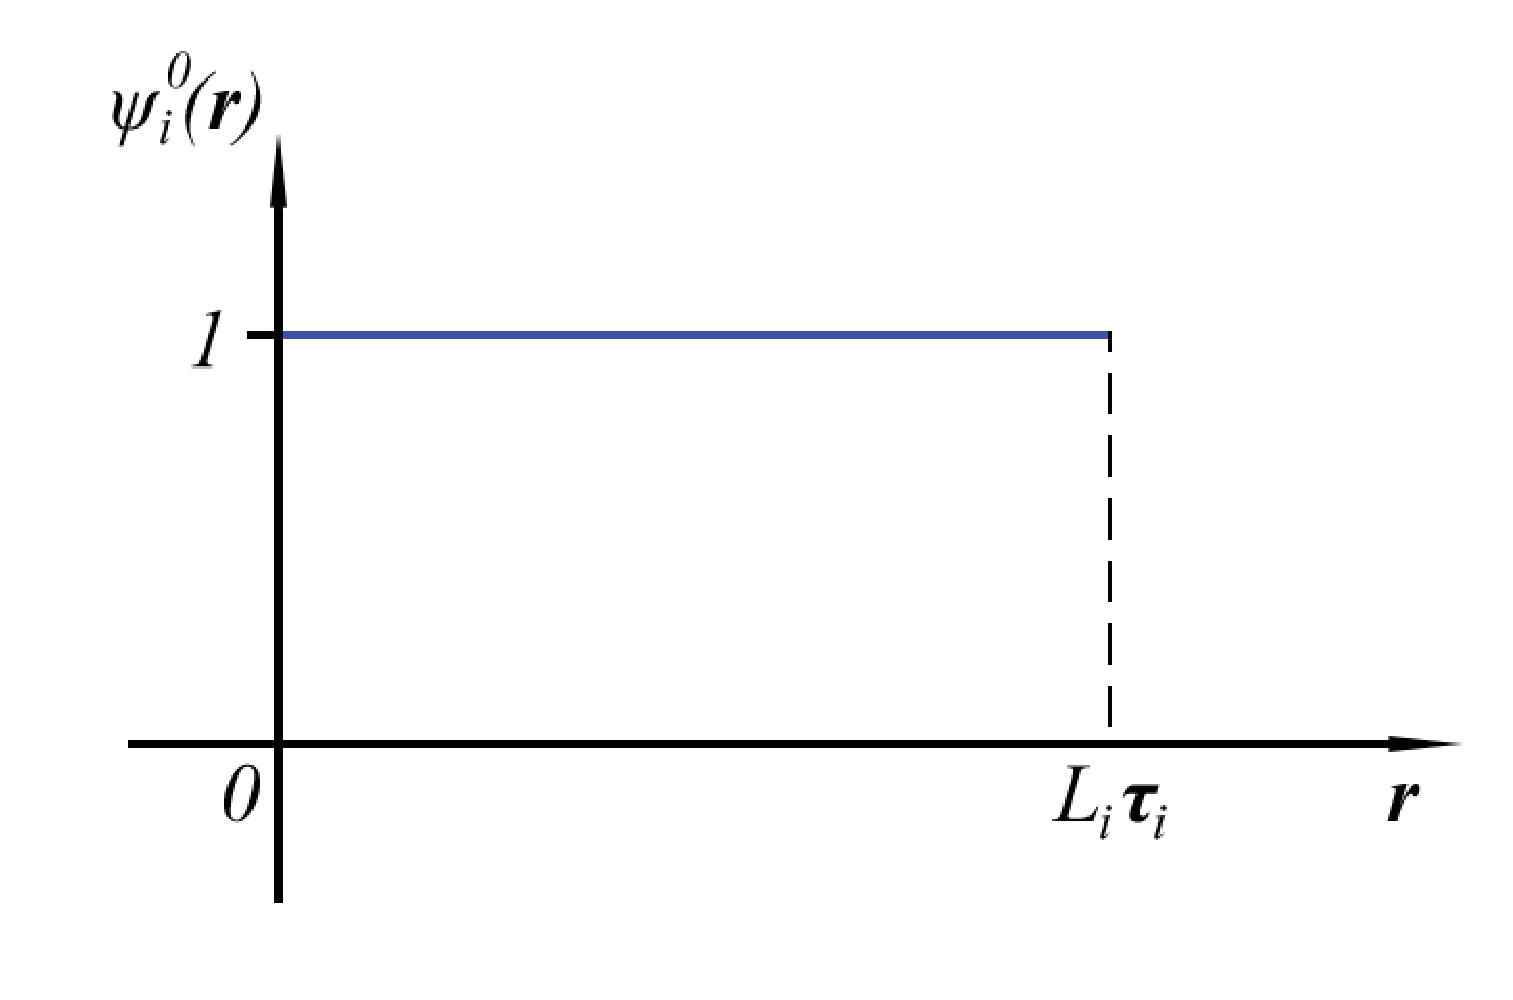
\includegraphics[width=0.9\textwidth]{phi0}
	\end{minipage}
	\begin{minipage}[h]{0.5\textwidth}
		\center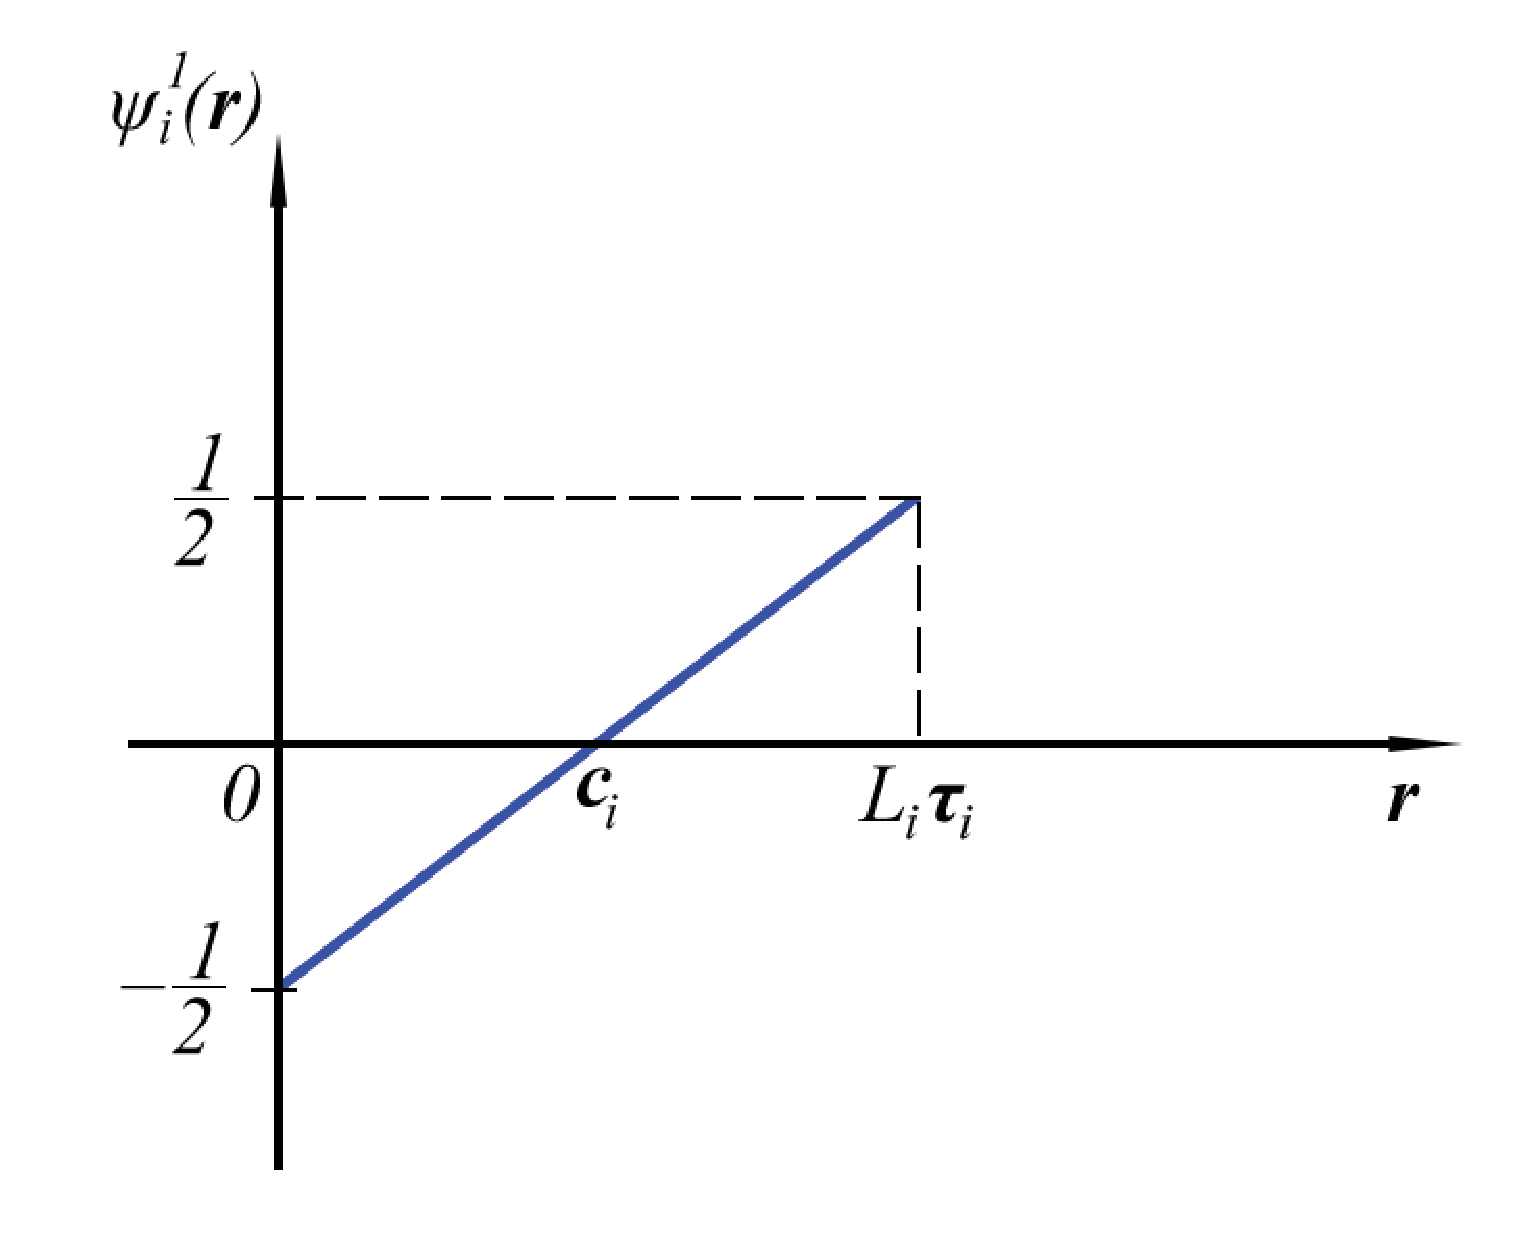
\includegraphics[width=0.9\textwidth]{phi1}
	\end{minipage}
\caption{Проекционные функции $\psi_i^0(\vec r)$ и $\psi_i^1(\vec r)$, совпадающие с базисными функциями $\varphi_i^0(\vec r)$ и $\varphi_i^1(\vec r)$ соответственно}\label{phi01}
\end{figure}
Тогда невязка уравнения~(\ref{Tscheme}) на каждой панели имеет вид
\begin{multline*}
p_i^1 (\vec r) = \sum_{j=1}^N \biggl(
\gamma_j^0 \int_{K_j} P_\tau \bigl( \vec r, \vec \xi \bigr) \varphi_j^0(\vec \xi) dl_\xi +
\gamma_j^1 \int_{K_j} P_\tau \bigl( \vec r, \vec \xi \bigr) \varphi_j^1(\vec \xi) dl_\xi
\biggr) - {} \\
{} -\frac 1 2 \bigl(\gamma_i^0 \varphi_i^0(\vec r) + \gamma_i^1 \varphi_i^1(\vec r) \bigr) - f_\tau(\vec r), \qquad \vec r \in K_i.
\end{multline*}

Коэффициенты при разложении $\{\gamma_i^0\}_{i=1}^N$ и $\{\gamma_i^1\}_{i=1}^N$,  согласно методу Галеркина~\cite{Fletcher}, будем искать из условий ортогональности невязки проекционным функциям, которые возьмем совпадающими с базисными функциями $\varphi_i^0(\vec r)$ и $\varphi_i^1(\vec r)$. Результирующие уравнения разделим на длины соответствующих панелей. 

Условие выделения единственного решения уравнения~\eqref{Circ2D} c учетом представления решения~\eqref{gamma1} имеет  вид
\[
\sum_{i=1}^N \int_{K_i}\bigl(\gamma_i^0 \varphi_i^0(\vec r) + \gamma_i^1 \varphi_i^1(\vec r) \bigr) dl_r = \Gamma^\ast.
\]

\looser{-0.02}{Таким образом, дискретным аналогом уравнения}~(\ref{Tscheme})\looser{-0.02}{ для расчетной схемы с кусочно-линейным представлением интенсивности} вихревого слоя является система линейных уравнений, включающая $(N+1)$ линейное уравнение относительно $N$ неизвестных $\{\gamma_i\}_{i=1}^N$. Для решения такой системы вводится регуляризирующая переменная~\cite{Lifanov}, и~в~результате решается система линейных алгебраических уравнений вида


\begin{equation}
\label{sys1}
\begin{pmatrix}
[A^{00}] + [D^{00}] & [A^{01}] + [D^{01}] & \{I_n\} \\
[A^{10}] + [D^{10}] & [A^{11}] + [D^{11}] & \{O_n\}\\
\{L^0\}^{\mathrm{T}} & \{L^1\}^{\mathrm{T}} & 0
\end{pmatrix}
\left(
\begin{array}{@{}c@{}}
\{\gamma^0\}\\
\{\gamma^1\}\\
R
\end{array}
\right)
=
\left(
\begin{array}{@{}c@{}}
\{b^0\} \\
\{b^1\}\\
\Gamma^\ast
\end{array}
\right),
\end{equation}
где блоки $[A^{pq}]$ --- квадратные матрицы размером $N\times N$; блоки $[D^{pq}]$ --- диагональные матрицы, $p,\,q = 0,\,1$; $\{L^0\}^{\mathrm{T}}$ и $\{L^1\}^{\mathrm{T}}$ --- $N$-мерные вектор-строки; $\{I_N\}$ --- столбец из единиц; $\{O_N\}$ ---столбец из нулей; $\{\gamma^0\}$ и $\{\gamma^1\}$ --- $N$-мерные векторы, составленные из искомых коэффициентов; $\{b^0\}$ и $\{b^1\}$ --- $N$-мерные векторы, образующие правую часть системы:
\begin{gather*}
A_{ij}^{pq} =\frac{1}{L_i}\int _{K_{i} }\biggl(\int _{K_{j} }P_\tau(\vec{r},\, \, \vec{\xi })\varphi _{j}^{q} (\vec{\xi })\, dl_{\xi }  \biggr) \, \varphi _{i}^{p} (\vec{r})\, dl_{r} ,\\[4mm]
D_{ii}^{pq} = -\frac 1{2L_i} \int_{K_i}\varphi_{i}^{p}(\vec r) \varphi_{i}^{q}(\vec r) dl_r, \quad L_i^p = \int_{K_i} \varphi_{i}^{p}(\vec r) dl_r, \\[4mm]
%D_{ii}^{0} =-\frac{L_{i} }{2}, \qquad  D_{ii}^{1} =-\frac{L_{i} }{24} ,\\[4mm]
b_{i}^{p} =\frac{1}{L_i}\int_{K_i}f_\tau(\vec{r}) \varphi_{i}^{p} (\vec{r})\, dl_{r} , \quad    p,\, q=0,\, 1,\quad   i,\, j=1,\,\ldots, \, N.
\end{gather*}

Учитывая, что $P_\tau(\vec{r},\, \, \vec{\xi }) = \vec n(\vec r) \cdot \vec Q(\vec{r}- \vec{\xi }),$ где
\[
	\vec Q(\vec r - \vec\xi) = \dfrac{\vec r-\vec\xi}{2\pi |\vec r-\vec\xi|^2},
\]
для компонент матриц $A^{pq}$ можно записать
\[
A_{ij}^{pq} = \frac{1}{L_i}\vec n_i \cdot \biggl(\underbrace{\int _{K_{i}} \varphi _{i}^{p} (\vec{r}) dl_{r} \int _{K_{j} } \vec Q(\vec{r}- \vec{\xi })\varphi _{j}^{q} (\vec{\xi })\, dl_{\xi }}_{\vec I^{pq}_{ij}} \biggr) = \frac{1}{L_i}\vec n_i \cdot \vec{I}_{ij}^{pq}.
\]
 Для компонент диагональных матриц $D^{pq}$ получаются выражения
\[
D_{ii}^{00} = -\frac {1}2, \qquad D_{ii}^{11} = -\frac {1}{24}, \qquad D_{ii}^{01} = D_{ii}^{10} = 0, \qquad i=1,\,\ldots, \, N,
\]
а коэффициенты векторов-строк $\{L^p\}^{\mathrm{T}}$ принимают значения
\[
L_i^0 = L_i, \qquad L_i^1 = 0, \qquad i=1,\,\ldots, \, N.
\]

\looser{-0.02}{Нахождение величин двойных интегралов, определяющих компоненты матриц}~$A^{pq}$, представляет собой основную сложность (здесь и далее под <<двойным интегралом>> понимается результат повторного вычисления криволинейных интегралов 1-го рода --- по  переменной $\vec r$, изменяющейся вдоль $i$-й панели, и по переменной $\vec\xi$, изменяющейся вдоль $j$-й панели).
Данные интегралы можно вычислить в общем виде для любых двух непересекающихся или имеющих общие концы отрезков $K_i$ и $K_j$ на плоскости; расчетные формулы приведены в статье~\cite{PMM}.

Компоненты векторов-столбцов правой части $\{b^0\}$ и $\{b^1\}$ линейной системы~\eqref{sys1} с~учетом движения профиля и отсутствия его деформации (за счет того, что длины панелей остаются неизменными) получаются интегрированием по панели скалярного произведения орта касательной и правой части~\eqref{f(r)} интегрального уравнения:
\[
b_i^p = \frac{1}{L_i} \int_{K_i} \bigl( \vec f(\vec r) \cdot \vec\tau(\vec r) \bigr) \varphi_i^p(\vec r)\, dl_r = (b_V)_i^p + \underbrace{(b_\Omega)_i^p}_0 + (b_{att})_i^p,
\]
где
\begin{gather*}
(b_V)_i^p = \frac{1}{L_i} \vec\tau_i \cdot \int_{K_i} \bigl( \alpha(\vec r) \vec U_K(\vec r) - \vec V_\infty \bigr) \varphi_i^p(\vec r)\, dl_r,\\[4mm]
(b_{att})_i^p = -\frac{1}{L_i} \vec\tau_i \cdot \int_{K_i} \biggl( \oint_{K} \frac{\vec k \times (\vec r - \vec \xi)}{2\pi|\vec r - \vec \xi|^2}\gamma^{att}(\vec\xi)\,dl_\xi
+\oint_{K} \frac{q^{att}(\vec \xi) (\vec r - \vec \xi)}{2\pi|\vec r - \vec \xi|^2}\,dl_\xi  \biggr)\varphi_i^p(\vec r)\, dl_r.
\end{gather*}

Далее запишем необходимые формулы для расчета всех возникающих интегралов в правой части матрицы системы $b_i^p$. Для члена $(b_V)_i^p$, определяемого скоростью набегающего потока, получаем
\begin{equation}
\label{VintUrect}
\left.
\begin{array}{@{}l@{}}
\displaystyle \int_{K_i} \bigl(\alpha(\vec r) \vec U_K(\vec r) - \vec V_\infty \bigr) \varphi_i^0(\vec r) dl_r = \Bigl( \frac12 \vec U_K (\vec c_i) - \vec V_\infty \Bigr) L_i,\\[4mm]
\displaystyle \int_{K_i} \bigl(\alpha(\vec r) \vec U_K(\vec r) - \vec V_\infty \bigr) \varphi_i^1(\vec r) dl_r = \frac{1}{12}\bigl(\vec U_K(\vec p_i) - \vec U_K(\vec c_i)\bigr) L_i,
\end{array}
\quad
\right\}
\end{equation}
где $\vec U_K(\vec c_i)$ и $\vec U_K(\vec p_i)$ --- скорости движения центра и начала $i$-й панели соответственно. При этом можно записать
\[
\vec U_K(\vec p_i) - \vec U_K(\vec c_i) = \frac12 \bigl( -\dot L_i \vec\tau_i + L_i \omega_i \vec n_i \bigr),
\]
где $\dot L_i$ --- скорость изменения длины $i$-й панели; $\omega_i$ --- ее угловая скорость; $\vec\tau_i$ --- как и ранее, орт касательной к панели, направленный от ее начала к концу; $\vec n_i$ --- орт внешней к профилю нормали. При этом предполагается, что обход профиля и нумерация панелей осуществляются таким образом, что при движении вдоль него область течения остается справа.

При вычислении вклада $(b_{att})_i^p$ в правую часть от слагаемых, выражающих влияние присоединенных слоев вихрей и источников, их интенсивности следует представлять в виде кусочно-линейных распределений --- согласованно с кусочно-линейным представлением решения:
\[
\begin{array}{@{}l@{}}
\displaystyle \gamma^{att}(\vec r) = \sum_{i=1}^N \bigl((\gamma^{att})_i^0 \varphi_i^0(\vec r) + (\gamma^{att})_i^1 \varphi_i^1(\vec r)\bigr);
\\
\displaystyle q^{att}(\vec r) = \sum_{i=1}^N \bigl((q^{att})_i^0 \varphi_i^0(\vec r) + (q^{att})_i^1 \varphi_i^1(\vec r)\bigr), \quad \vec r \in K.
\end{array}
\]
Для определения коэффициентов $(\gamma^{att})_i^p$ и $(q^{att})_i^p$ следует знать скорость движения центра панели $\vec U_K(\vec c_i)$, угловую скорость ее вращения $\omega_i$ и скорость изменения длины $\dot L_i$, тогда
\[
\begin{array}{@{}l@{\qquad}l@{}}
(\gamma^{att})_i^0 = \vec U_K(\vec c_i) \cdot \vec \tau_i,  &
(\gamma^{att})_i^1 = \dot L_i,\\
(q^{att})_i^0 = \vec U_K(\vec c_i) \cdot \vec n_i,  &
(q^{att})_i^1 = -L_i \omega_i.
\end{array}
\]

Следовательно, два интеграла в слагаемом $(b_{att})_i^p$ можно выразить через ранее введенные величины $\vec I_{ij}^{pq}$:
\[
\begin{array}{@{}l@{}}
\displaystyle \int_{K_i}  \varphi _{i}^{p} (\vec{r}) dl_r \oint_{K} \frac{\vec k \times (\vec r - \vec \xi)}{2\pi|\vec r - \vec \xi|^2}\gamma^{att}(\vec\xi)\,dl_\xi = \vec k \times  \sum\limits_{j=1}^N \Bigl(\vec I_{ij}^{p0} (\gamma^{att})_j^0 + \vec I_{ij}^{p1} (\gamma^{att})_j^1 \Bigr),\\
\displaystyle \int_{K_i}  \varphi _{i}^{p} (\vec{r}) dl_r \oint_{K} \frac{q^{att}(\vec\xi) (\vec r - \vec \xi)}{2\pi|\vec r - \vec \xi|^2} dl_\xi = \sum\limits_{j=1}^N \Bigl(\vec I_{ij}^{p0} (q^{att})_j^0 + \vec I_{ij}^{p1} (q^{att})_j^1 \Bigr).
\end{array}
\]

Построенную $T$-схему с кусочно-линейным представлением решения интегрального уравнения~\eqref{Tscheme}, выражаемую системой линейных алгебраических уравнений~\eqref{sys1}, будем обозначать $\mathcal{T}^1$, а $T$-схему с кусочно-постоянным представлением решения, т.\,е.
\[
	\label{gamma0}
	\gamma(\vec r) = \sum_{i=1}^N \gamma_i^0 \varphi_i^0(\vec r), \quad \vec r \in K,
\]
будем обозначать как  $\mathcal{T}^0$.


Далее на Рис.~\ref{wing100boundSol_toYuliya}--\ref{wing100unboundSol_toYuliya} представлены результаты работы кусочно-линейной и кусочно-постоянной схем для численного решения граничного интегрального уравнения~\eqref{Tscheme} относительно интенсивности вихревого слоя в сравнении с известным точным решением.

\begin{figure}[!h]
	\center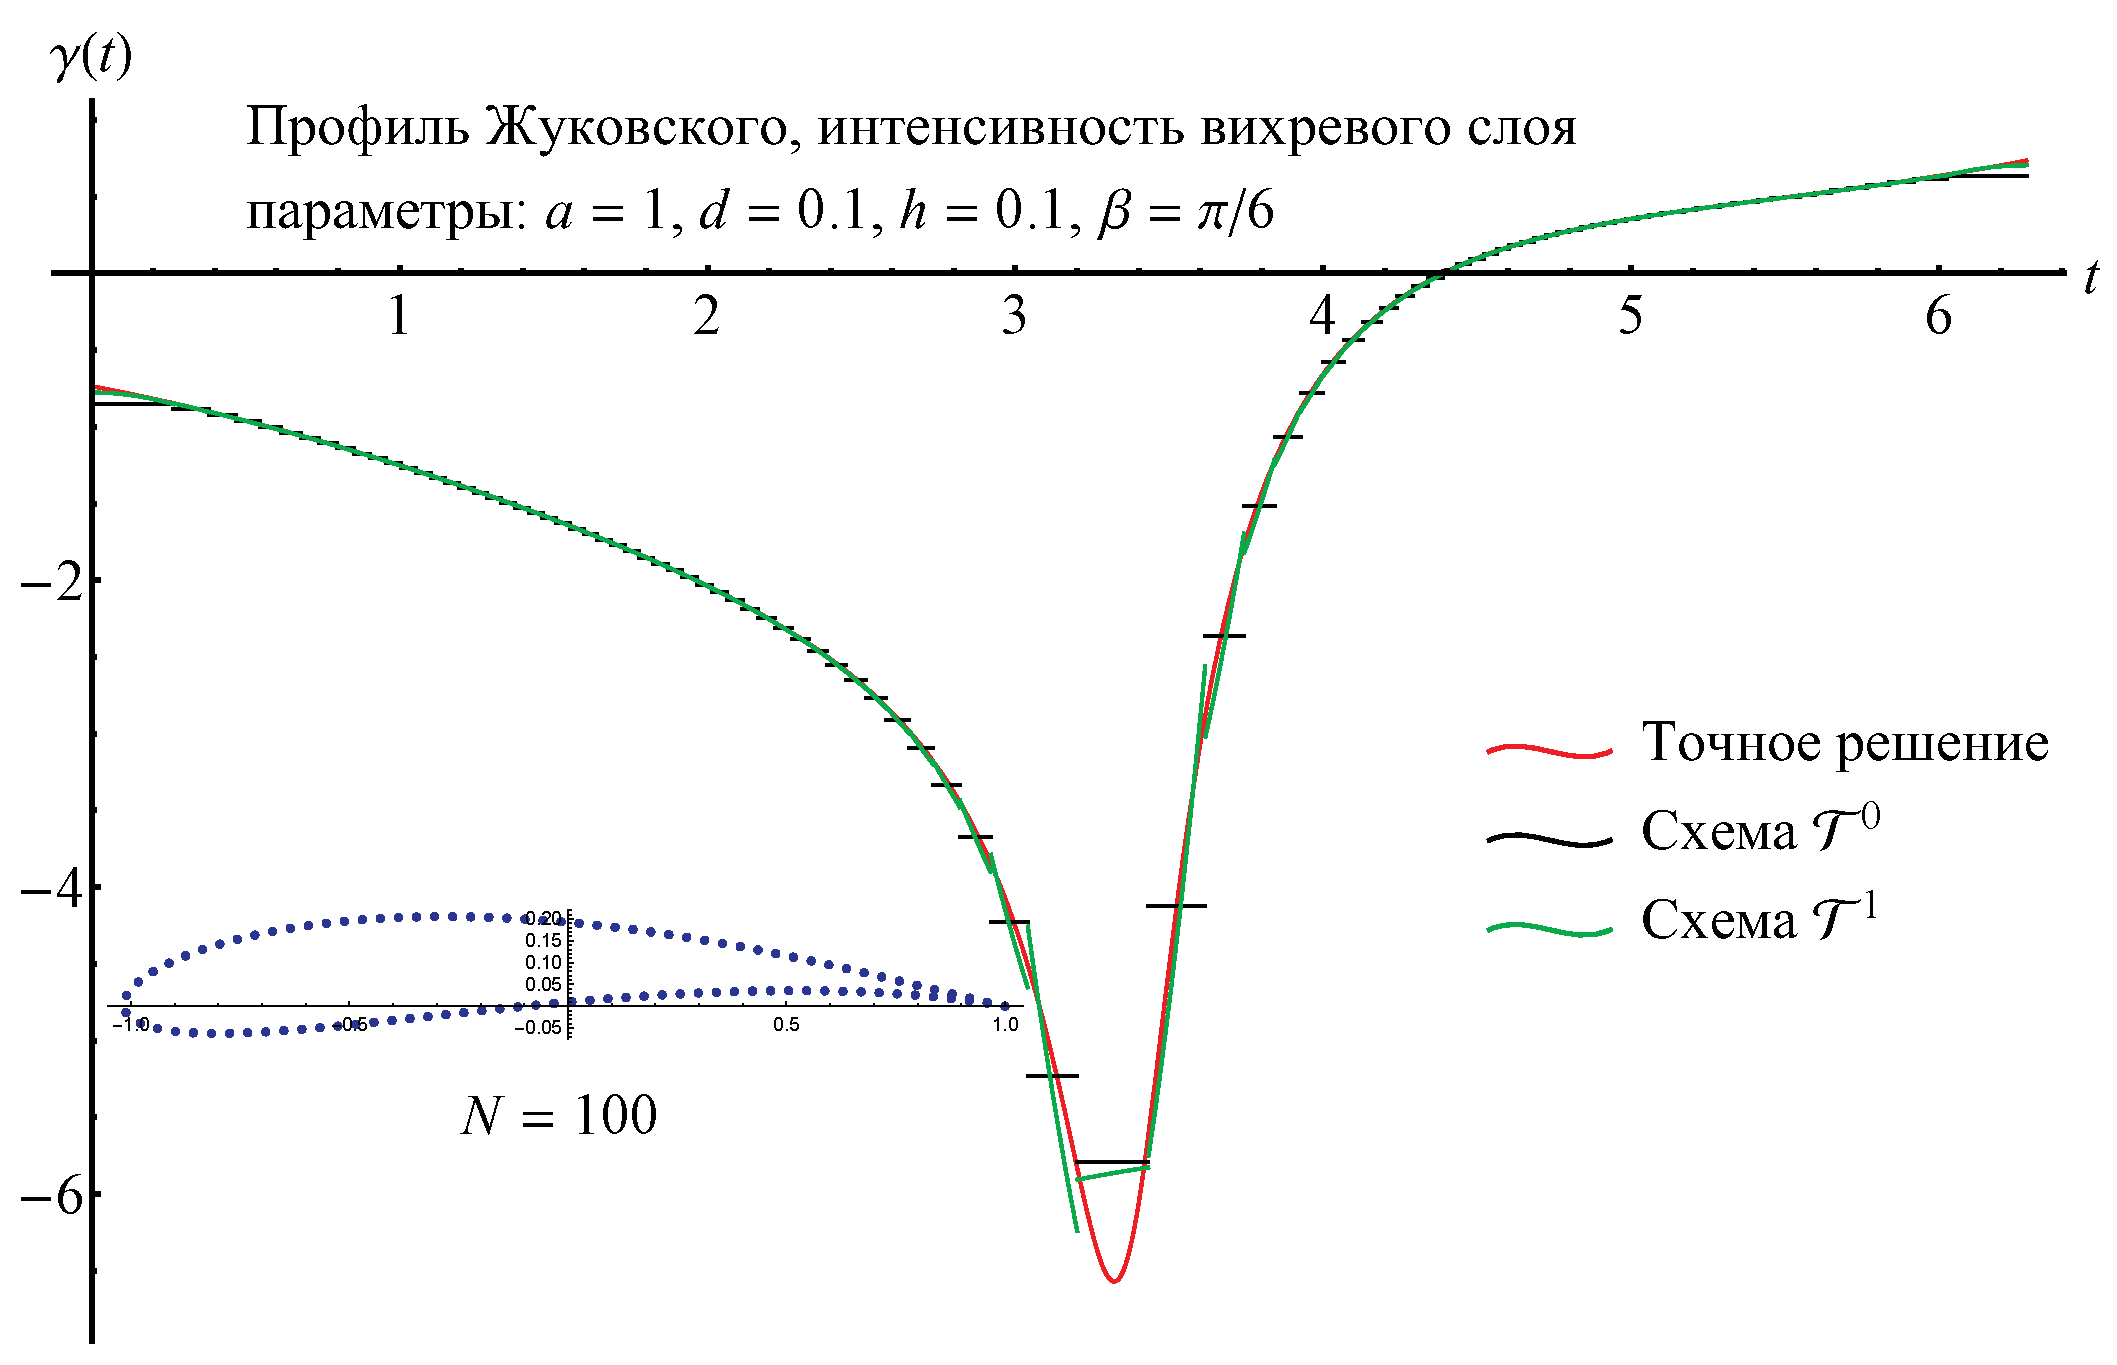
\includegraphics[width=0.85\textwidth]{wing100boundSol_toYuliya}
	\caption{Результат применения схем с кусочно-постоянным и кусочно-линейным представлениями решения для случая стационарного обтекания крыла}\label{wing100boundSol_toYuliya}
\end{figure}

\begin{figure}[!h]
	\center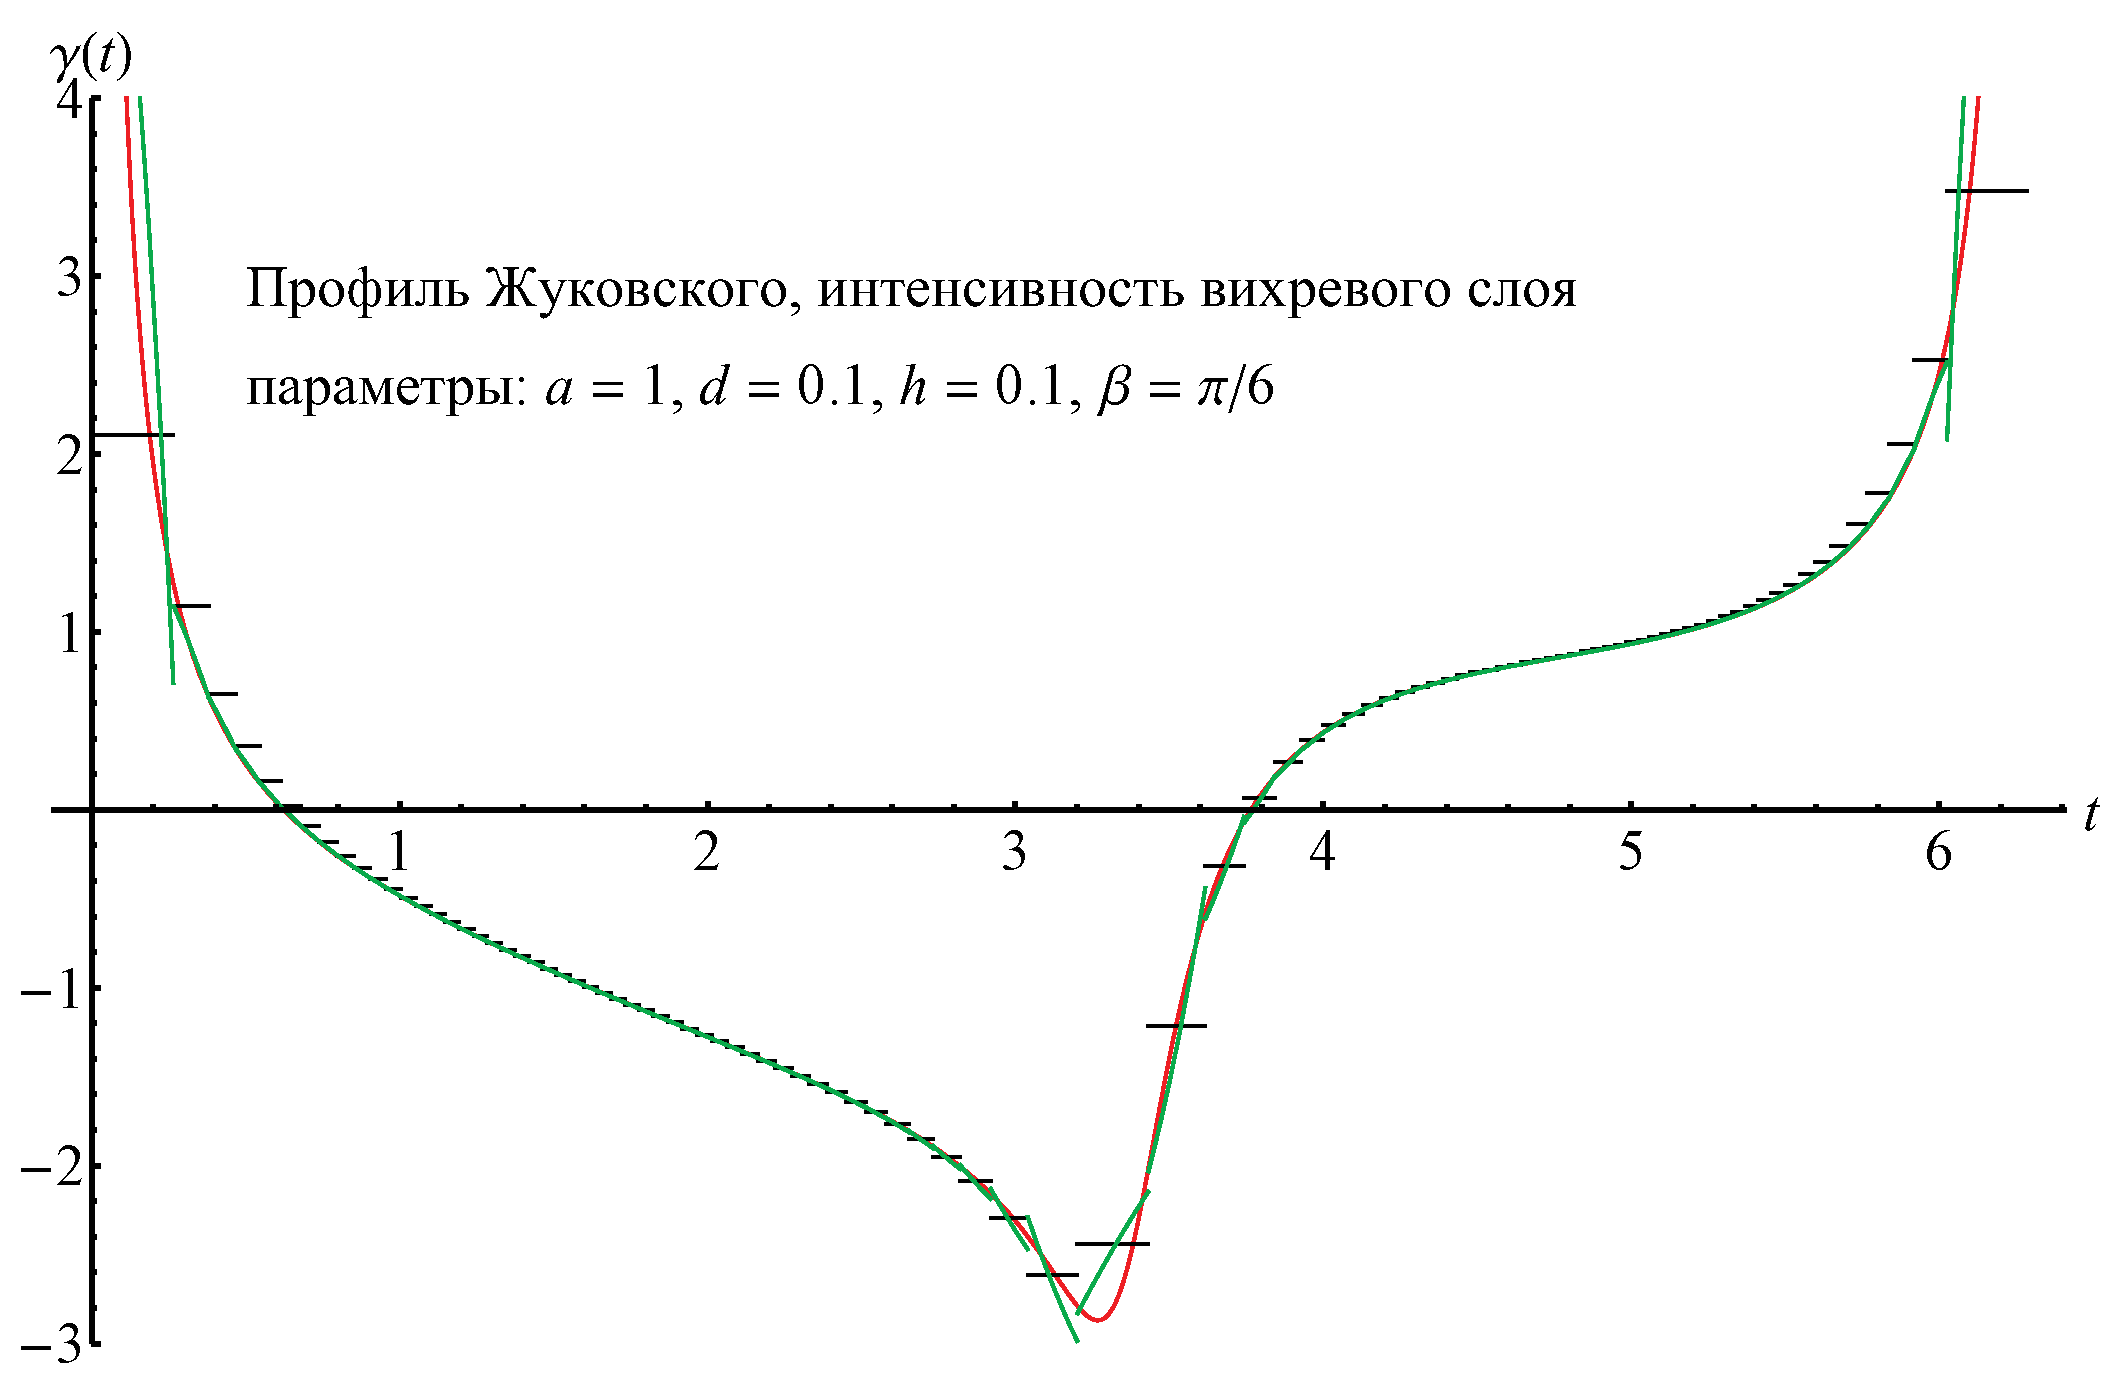
\includegraphics[width=0.85\textwidth]{wing100unboundSol_toYuliya}
	\caption{Результат применения схем с кусочно-постоянным и кусочно-линейным представлениями решения для случая нестационарного обтекания крыла}\label{wing100unboundSol_toYuliya}
\end{figure}\medskip

По построению кусочно-постоянная схема имеет 1-й порядок точности, а кусочно-линейная схема --- 2-й порядок. При этом видно, что использование кусочно-постоянной и кусочно-линейной схем на крайних панелях на Рис.~\ref{wing100unboundSol_toYuliya} приводит к очень большой погрешности при воспроизведении точного решения. Это связано с тем, что решение в данном случае является неограниченным, что и приводит к потере 1-го и 2-го порядков точности для обеих схем. 

\subsection{$T$-схема с асимптотическим решением вблизи острой кромки}

При рассмотрении обтекания профиля с угловыми точками, угол при которых (со стороны области течения) больше развернутого, интенсивность вихревого слоя при приближении к ним неограниченно возрастает; в монографии~\cite{Lifanov} указано, что имеет место асимптотика решения
\begin{equation}
\label{asympgamma}
\gamma(\rho) \sim \frac{1}{\rho^\mu},
\end{equation}
где $\mu = 1-\pi/\chi$; $\chi > \pi$ --- внешний угол; $\rho$ --- расстояние до угловой точки.

К примеру, для обобщенного профиля Жуковского с параметрами $a=1$, $d=0.1$, $h=0.1$, $\sigma = 15/8$
с углом при острой кромке
$\beta = (2-\sigma)\pi = \pi/8$
и внешним углом\linebreak $\chi=\sigma\pi = 15\pi/8$, установленного под углом атаки $\alpha = {\pi}/{6}$ к набегающему потоку единичной скорости, при задании циркуляции $\Gamma = 0$ на Рис.~\ref{FigExAsPrmLog} в двойном логарифмическом масштабе показан график точного решения для интенсивности вихревого слоя на первых трех панелях (нумерация панелей идет от острой кромки против часовой стрелки) в зависимости от расстояния до кромки. Границам панелей соответствуют вертикальные линии сетки; по причине логарифмического масштаба основная часть графика соответствует 1-й панели. Штриховой линией показала зависимость~\eqref{asympgamma}, для данного примера $\mu = \sfrac7{15}$.

\begin{figure}[!h]
	\centering
	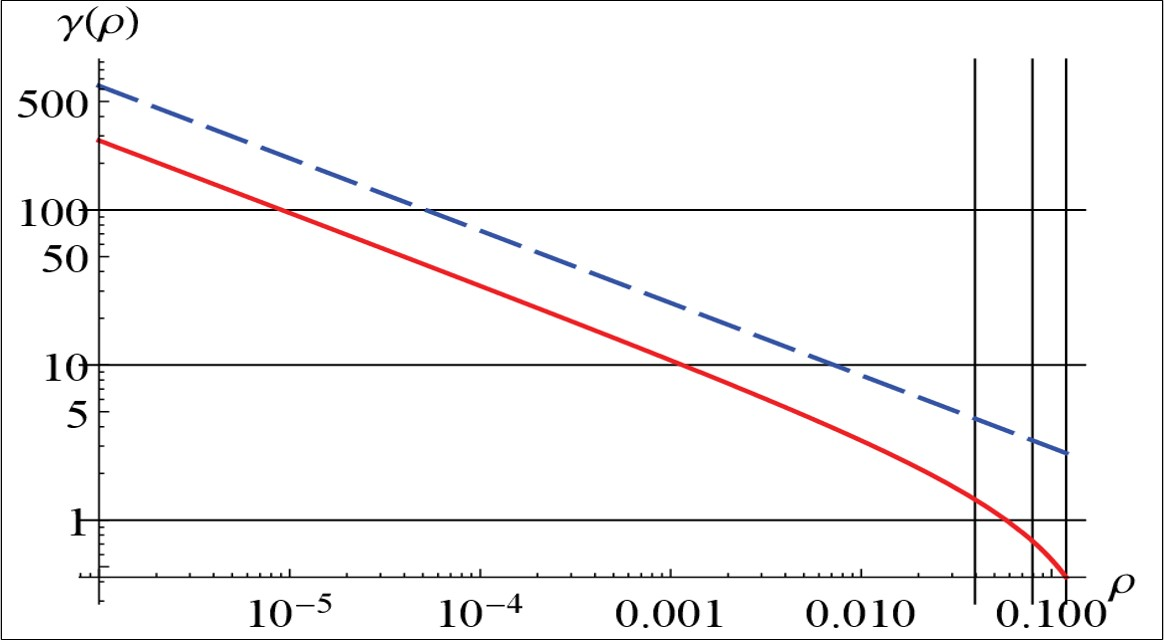
\includegraphics[width=0.70\textwidth]{ris11}%
	\caption{\label{FigExAsPrmLog}Интенсивность вихревого слоя на первых трех панелях обобщенного профиля Жуковского в зависимости от расстояния до острой кромки в сравнении с зависимостью~\eqref{asympgamma}}
	\vspace*{-2mm}
\end{figure}

Из Рис.~\ref{FigExAsPrmLog} видно, что точное решение на 1-й панели практически  пропорционально функции $\rho^{-\mu}$. 

Знание асимптотического поведения решения на панелях, примыкающих к угловой точке, позволяет построить более точную $T$-схему для численного решения, используя описанную ранее процедуру Галеркина. Для
этого на всех панелях, кроме примыкающих к угловой точке (т.\,е.\ панелей с~индексами $1$ и $N$ для рассматриваемого примера) решение, как и ранее, представляется линейной комбинацией базисных функций $\varphi^0_i(\vec r)$ и $\varphi^1_i(\vec r)$, $i=2,\,\ldots,\,N-1$, тогда как на двух выделенных панелях --- комбинацией базисных функций $\varphi^0_1(\vec r)$, $\varphi^1_1(\vec r)$, $\varphi^a_1(\vec r)$ и $\varphi^0_N(\vec r)$, $\varphi^1_N(\vec r)$, $\bar\varphi^a_N(\vec r)$ соответственно:
\begin{multline}
\label{asympsol}
\gamma(\vec r) = \sum\limits_{i=2}^{N-1} \bigl( \gamma_i^0 \varphi_i^0(\vec r) + \gamma_i^1 \varphi_i^1(\vec r) \bigr) + \bigl( \gamma_1^0 \varphi_1^0(\vec r) + \gamma_1^1 \varphi_1^0(\vec r) + \gamma_1^a \varphi_1^a(\vec r) \bigr) + {}\\
{} + \bigl( \gamma_N^0 \varphi_N^0(\vec r) + \gamma_N^1 \varphi_1^0(\vec r) + \gamma_N^a \bar\varphi_N^a(\vec r) \bigr),
\end{multline}
где, как и ранее, $\varphi^0_1(\vec r)$ и $\varphi^0_N(\vec r)$ --- функции-индикаторы $1$-й и $N$-й панелей соответственно, $\varphi^1_1(\vec r)$ и $\varphi^1_N(\vec r)$ --- кусочно-линейные базисные функции, а новые базисные функции $\varphi^a_1(\vec r)$ и $\bar\varphi^a_N(\vec r)$ принимают значения:
\begin{equation}
\label{asympbasis}
\left.
\begin{array}{@{}l@{}}
\displaystyle \varphi^a_1(\vec r) = \frac{L_1^\mu}{s_1(\vec r)^\mu} - \frac{1}{1-\mu}, \\[5mm]
\displaystyle \bar\varphi^a_N(\vec r) = \frac{L_N^\mu}{\bigl(L_N-s_N(\vec r)\bigr)^\mu} - \frac{1}{1-\mu}.
\end{array}
\qquad
\right\}
\end{equation}
Здесь $s_i(\vec r) =(\vec r - \vec p_i)\cdot\vec\tau_i$ --- расстояние, измеряемое вдоль $i$-й панели от ее начала~$\vec p_i$; $\mu$ --- показатель степени, определяющий асимптотическое поведение решения~\eqref{asympgamma}, остальные обозначения идентичны использованным ранее. Разница между функциями $\varphi(\vec r)$ и $\bar\varphi(\vec r)$ заключается в <<ориентации>> особенности: в первом случае она имеет место в начале панели, во втором --- на конце.
Постоянные слагаемые в функциях~\eqref{asympbasis} выбраны таким образом, чтобы обеспечить условие их ортогональности постоянным базисным функциям:
\[
\int_{K_1} \varphi_1^0(\vec r) \varphi_1^a(\vec r) \, dl_r = \int_{K_N} \varphi_N^0(\vec r) \bar\varphi_N^a(\vec r) \, dl_r =0.
\]

Для определения неизвестных коэффициентов разложения приближенного решения~\eqref{asympsol} по базисным функциям будем, как и ранее, рассматривать условие ортогональности невязки системе проекционных функций.
В ранее построенных $T$-схемах во всех случаях в качестве проекционных использовался набор базисных функций, однако в данном случае это вызывает излишние сложности при вычислении коэффициентов результирующей системы линейных уравнений, поэтому теперь в дополнение к проекционным функциям, выбранным как и в предыдущем разделе, введем новые проекционные базисные функции на крайних панелях $\psi_1^2(\vec r)$ и $\psi_N^2(\vec r)$:
\begin{equation}
\label{psi2}
	\psi_i^2(\vec r)=2\left|\frac{(\vec r -\vec c_i)\cdot\vec\tau_i}{L_i}\right|-\frac{L_i}{2},\qquad i=1,\,N.
\end{equation}

\begin{figure}[!h]
	\centering
	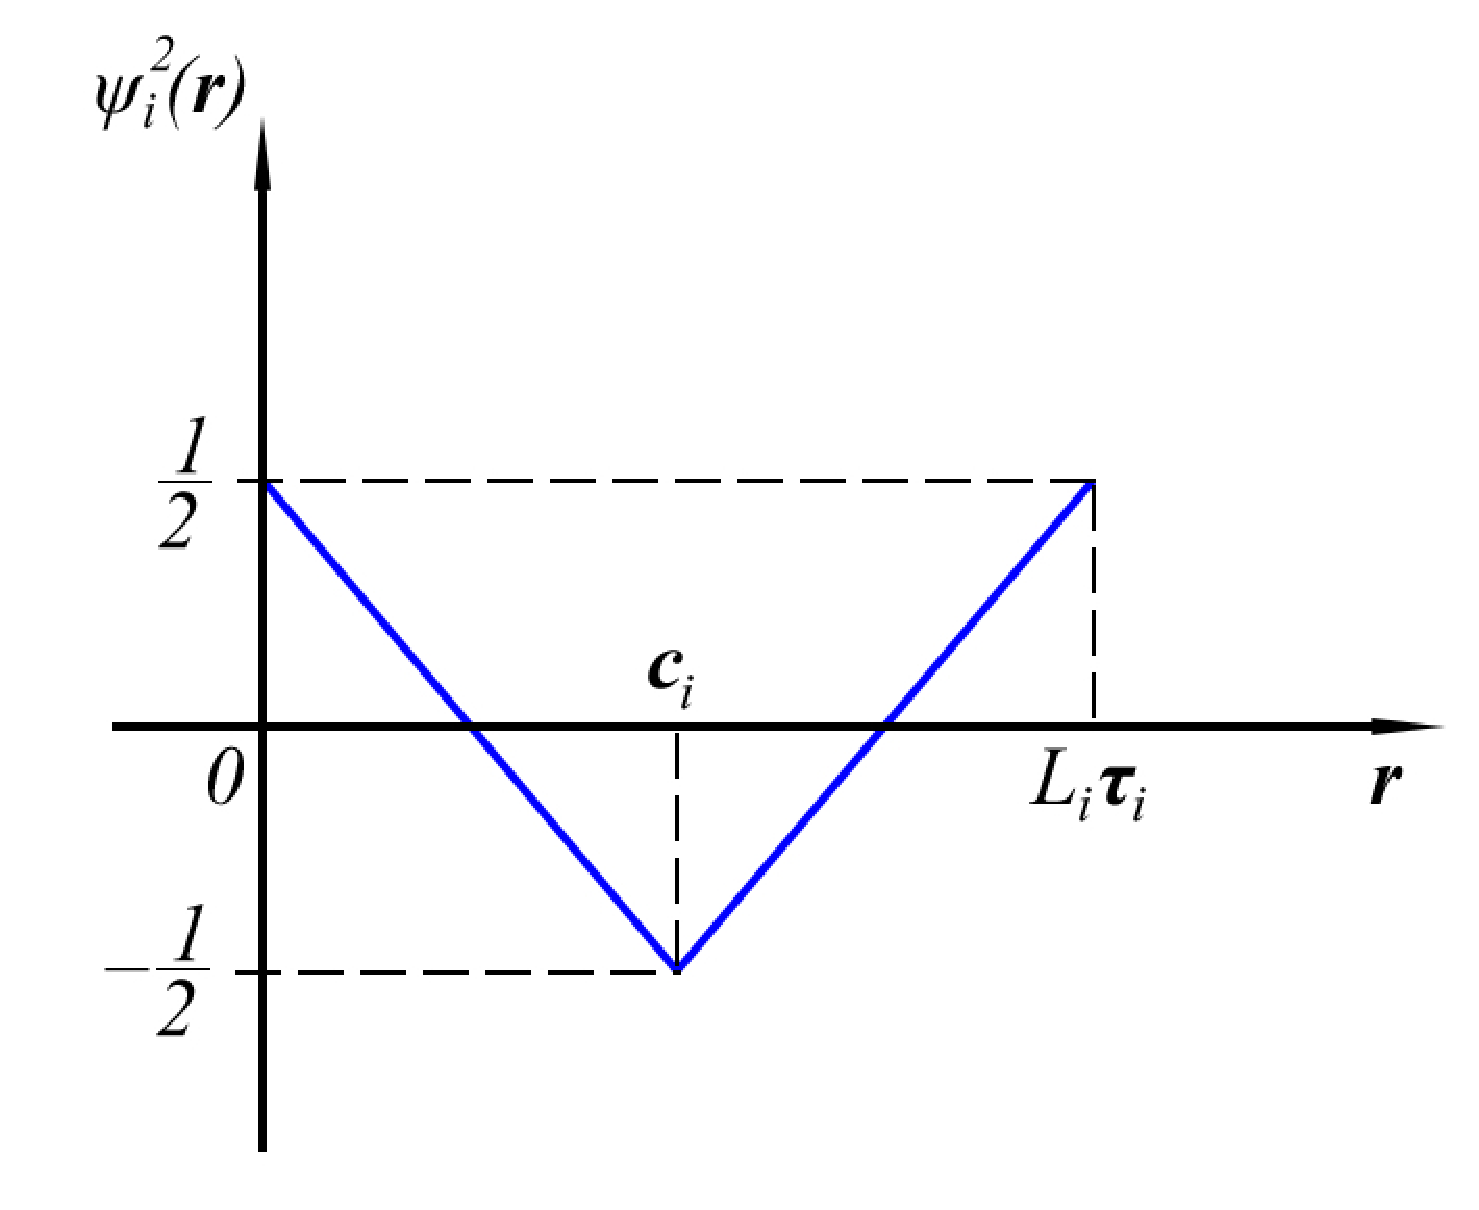
\includegraphics[width=0.5\textwidth]{phi2}%
	\caption{\label{phi2}Проекционная функция $\psi_i^2(\vec r)$, $i=1,\,N$}
	\vspace*{-2mm}
\end{figure}

Обозначим такую схему $\mathcal{T}^1_{aMOD}$; ее можно рассматривать как результат применения известного метода Петрова --- Галеркина.

Получаемая в результате система линейных уравнений, соответствующая схеме $\mathcal{T}^1_{aMOD}$, принимает вид
\begin{equation}
\label{sys1asymp}
\left(
\begin{array}{@{}ccccc@{}}
[A^{00}] + [D^{00}] & [A^{01}] + [D^{01}] & \{A^{0,\,a}_{i,\,1}\} & \{A^{0,\,a}_{i,\,N}\} & \{I_N\} \\
{[}A^{10}{]} + [D^{10}] & [A^{11}] + [D^{11}] & \{A^{1,\,a}_{i,\,1}\} & \{A^{1,\,a}_{i,\,N}\} & \{O_N\} \\
\{A^{20}_{1,j}\}^\mathrm{T} &\{A^{21}_{1,j}\}^\mathrm{T} & D_{11}^{2,a} &  A^{2,a}_{1N} & 0\\
\{A^{20}_{N,j}\}^\mathrm{T} & \{A^{21}_{N,j}\}^\mathrm{T} & A^{2,a}_{N1} & D_{NN}^{2,a} & 0\\
\{L^0\}^\mathrm{T} & \{L^1\}^\mathrm{T} & 0 & 0 & 0
\end{array}
\right)
\left(
\begin{array}{@{}c@{}}
\{\gamma^0\} \\
\{\gamma^1\} \\
\gamma^a_1\\
\gamma^a_N\\
R
\end{array}
\right)
=
\left(
\begin{array}{@{}c@{}}
\{b^0\} \\
\{b^1\} \\
b^a_1\\
b^a_N\\
\Gamma
\end{array}
\right),
\end{equation}
и имеет размерность $(2N+3)$. Данная система образована путем добавления к матрице левой части системы~\eqref{sys1} двух строк и двух столбцов, а к правой части системы~\eqref{sys1} --- двух элементов $b^a_1$ и $b^a_N$, что соответствует введению двух новых базисных и проекционных функций на крайних панелях. Здесь, как и ранее, блоки $[A^{pq}]$ --- квадратные матрицы размером $N\times N$; блоки $[D^{pq}]$ --- диагональные матрицы, $p,\,q = 0,\,1$; $\{L^0\}^{\mathrm{T}}$ и $\{L^1\}^{\mathrm{T}}$ --- $N$-мерные вектор-строки; $\{I_N\}$ --- столбец из единиц; $\{O_N\}$ ---столбец из нулей; $\{\gamma^0\}$ и $\{\gamma^1\}$ --- $N$-мерные векторы, составленные из искомых коэффициентов; $\{b^0\}$ и $\{b^1\}$ --- $N$-мерные векторы, образующие правую часть системы,а коэффициенты векторов-строк $\{L^p\}^{\mathrm{T}}$ принимают те же значения. Добавленные компоненты $N$-мерных векторов $\{A_{i,1}^{p,a}\}$ могут быть вычислены по формулам:

\begin{multline}
\label{longIntegral}
A_{i,1}^{p,a} =\frac{1}{L_i}\int _{K_{i} }\biggl(\int_{K_{1} }P_\tau(\vec{r},\, \vec{\xi })\varphi_1^{a} (\vec{\xi })\, dl_{\xi }  \biggr) \, \varphi _{i}^{p} (\vec{r})\, dl_{r} = {}\\[5mm]
{}=\frac{1}{L_i} \Biggl( \int _{K_{i} }\biggl(\int_{K_{1} } \bigl(\vec n(\vec r) \cdot \vec Q(\vec{r}- \vec{\xi })\bigr) \frac{L_1^\mu}{s_1(\vec \xi)^\mu}\, dl_{\xi }  \biggr) \, \varphi _{i}^{p} (\vec{r})\, dl_{r} - {}\\[5mm]
{} \qquad {} 
- \frac{1}{1-\mu} \int _{K_{i} }\biggl(\int_{K_{1} } \bigl(\vec n(\vec r) \cdot \vec Q(\vec{r}- \vec{\xi })\bigr)\, dl_{\xi }  \biggr) \, \varphi _{i}^{p} (\vec{r})\, dl_{r} \Biggr) = {}\\[5mm]
{} = \frac{1}{L_i} \biggl( \bigl(\vec n_i \cdot \vec H_{i,1}^{p,1}\bigr) - \frac{1}{1-\mu} \bigl(\vec n_i \cdot \vec I_{i,1}^{p,0}\bigr) \biggr), \qquad p=0,\,1.
\end{multline}

Задача сводится, таким образом, к~вычислению интегралов, обозначенных как $\vec H_{i,1}^{p,1}$ и предполагающих интегрирование неограниченной функции $\Bigl(\sfrac{L_1}{s_1(\vec \xi)}\Bigr)^{\mu}$, где $s_1(\vec \xi)$ --- расстояние от начала $1$-й панели~\cite{Marchevskii}.

Получим выражения для компонент векторов $A_{1,1}^{1,a}$ и $A_{N,N}^{1,a}$, а также для коэффициентов $D_{11}^{2,a}$ и $D_{NN}^{2,a}$.
Они выражаются интегралами от произведения базисной функции на проекционную и могут быть вычислены в~замкнутой форме:
\[
\begin{array}{@{}l@{}}
\displaystyle A_{11}^{1,a} = -\frac{1}{2L_1} \int_{K_1} \varphi_1^1(\vec r)\varphi_1^a(\vec r) dl_r = \frac{\mu}{4(\mu^2 - 3\mu + 2)},\\[5mm]
\displaystyle A_{NN}^{1,a} = -\frac{1}{2L_N} \int_{K_N} \varphi_N^1(\vec r)\bar\varphi_N^a(\vec r) dl_r =- \frac{\mu}{4(\mu^2 - 3\mu + 2)},\\[5mm]
\displaystyle D_{11}^{2,a} = -\frac{1}{2L_1} \int_{K_1} \psi_1^2(\vec r)\varphi_1^a(\vec r) dl_r = \frac{\mu-2^{\mu+1}+2}{4(\mu^2 - 3\mu + 2)},\\[5mm]
\displaystyle D_{NN}^{2,a} = -\frac{1}{2L_N} \int_{K_N} \psi_N^2(\vec r)\bar\varphi_N^a(\vec r) dl_r =\frac{\mu-2^{\mu+1}+2}{4(\mu^2 - 3\mu + 2)}.
\end{array}
\]



Запишем выражения для вычисления компонент векторов-строк $\{ A^{20}_{1,j}\}^\mathrm{T}$, $\{ A^{20}_{N,j}\}^\mathrm{T}$: 
\[
\begin{array}{@{}l@{}}
\displaystyle A^{20}_{1,j} = \frac{1}{L_1} \int_{K_1} \psi_1^2(\vec r) dl_r\int_{K_j}\varphi_j^0(\vec \xi)P_\tau(\vec{r},\, \, \vec{\xi }) dl_{\xi },\\[5mm]
\displaystyle A^{20}_{N,j} = \frac{1}{L_N} \int_{K_N} \psi_N^2(\vec r) dl_r\int_{K_j}\varphi_j^0(\vec \xi)P_\tau(\vec{r},\, \, \vec{\xi }) dl_{\xi },
\end{array}
\]
и  для $\{ A^{21}_{1,j}\}^\mathrm{T}$, $\{ A^{21}_{N,j}\}^\mathrm{T}$:
\[
\begin{array}{@{}l@{}}
\displaystyle A^{20}_{1,j} = \frac{1}{L_1} \int_{K_1} \psi_1^2(\vec r) dl_r\int_{K_j}\varphi_j^1(\vec \xi)P_\tau(\vec{r},\, \, \vec{\xi }) dl_{\xi },\\[5mm]
\displaystyle A^{20}_{N,j} = \frac{1}{L_N} \int_{K_N} \psi_N^2(\vec r) dl_r\int_{K_j}\varphi_j^1(\vec \xi)P_\tau(\vec{r},\, \, \vec{\xi }) dl_{\xi }.
\end{array}
\]

Соответственно, коэффициенты $A^{2,a}_{1N}$ и $A^{2,a}_{N1}$ можно записать следующим образом:
\[
\begin{array}{@{}l@{}}
\displaystyle A^{2,a}_{1N} = \frac{1}{L_1} \int_{K_1} \psi_1^2(\vec r) dl_r\int_{K_N}\varphi_N^a(\vec \xi)P_\tau(\vec{r},\, \, \vec{\xi }) dl_{\xi },\\[5mm]
\displaystyle A^{2,a}_{N1} = \frac{1}{L_N} \int_{K_N} \psi_N^2(\vec r) dl_r\int_{K_1}\varphi_1^a(\vec \xi)P_\tau(\vec{r},\, \, \vec{\xi }) dl_{\xi }.
\end{array}
\]

Все описанные выше интегралы можно найти численно, используя методику, описанную в\cite{Marchevskii}. 
%и по форме совпадает с системой~\eqref{sys1}, полученной в разделе~\ref{sec25} для схемы $\mathcal{T}^1$ при кусочно-линейном представлении решения.
\subsection{Упрощенный вариант $T$-схемы с асимптотическим решением}

Рассмотрим упрощенный вариант реализации $T$-схемы с асимптотическим решением. Теперь будем считать, что на всех панелях, кроме примыкающих к угловой точке, решение представляется линейной комбинацией базисных функций $\varphi^0_i(\vec r)$ и~$\varphi^1_i(\vec r)$, $i=2,\,\ldots,\,N-1$, а на двух выделенных крайних панелях --- комбинацией базисных функций $\varphi^0_1(\vec r)$, $\varphi^a_1(\vec r)$ и $\varphi^0_N(\vec r)$, $\bar\varphi^a_N(\vec r)$ соответственно:
\begin{multline}
\label{asympsollight}
\gamma(\vec r) = \sum\limits_{i=2}^{N-1} \bigl( \gamma_i^0 \varphi_i^0(\vec r) + \gamma_i^1 \varphi_i^1(\vec r) \bigr) + {}\\
{} + \bigl( \gamma_1^0 \varphi_1^0(\vec r) + \gamma_1^a \varphi_1^a(\vec r) \bigr) +
\bigl( \gamma_N^0 \varphi_N^0(\vec r) + \gamma_N^a \bar\varphi_N^a(\vec r) \bigr).
\end{multline}

В~качестве проекционных функций выберем базисные функции схемы~$\mathcal{T}^1$ с~кусочно-линейным решением, т.\,е.\ набор функций $\{\varphi_i^0(\vec r)\}_{i=1}^N$, $\{\varphi_i^1(\vec r)\}_{i=1}^{N}$.
Обозначим такую схему $\mathcal{T}^1_a$. 

Получаемая для определения неизвестных коэффициентов разложения система линейных уравнений, соответствующая схеме $\mathcal{T}^1_a$, принимает вид
\begin{equation}
\label{sys1asymplight}
\left(
\begin{array}{@{}ccc@{}}
[A^{00}] + [D^{00}] & [A^{01}] + [D^{01}] & \{I_N\} \\
{[}A^{10}{]} + [D^{10}] & [A^{11}] + [D^{11}] & \{O_N\} \\
\{L^0\}^\mathrm{T} & \{L^1\}^\mathrm{T} & 0
\end{array}
\right)
\left(
\begin{array}{@{}c@{}}
\{\gamma^0\} \\
\{\gamma^1\} \\
R
\end{array}
\right)
=
\left(
\begin{array}{@{}c@{}}
\{b^0\} \\
\{b^1\} \\
\Gamma
\end{array}
\right),
\end{equation}
и по форме совпадает с системой~\eqref{sys1}, полученной для схемы $\mathcal{T}^1$ при кусочно-линейном представлении решения. Более того, с учетом определения коэффициентов системы~\eqref{sys1}, можно заключить, что все они остаются неизменными за исключением первых и последних столбцов блоков $[A^{01}]$ и $[A^{11}]$, для вычисления компонент которых справедлива формула~\eqref{longIntegral}, а также первого и~последнего диагональных коэффициентов в блоке $[D^{11}]$, совпадающих с коэффициентами $ A_{11}^{1,a}$ и $ A_{NN}^{1,a}$ по построению соответственно.

Сравнивая две представленные численные схемы с асимптотическим представлением решения на острой кромке, можно заметить, что в упрощенном варианте получаемая система линейных алгебраических уравнений имеет размерность $(2N+1)$, в то время, как первая из описанных схем с асимптотическим представлением решения имеет размерность $(2N+3)$. Стоит отметить, что введение новой проекционной базисной функции сопровождается большим количеством необходимых для составления системы интегралов, вычисление которых усложняет процесс в целом. Следовательно, необходимо оценить рациональность введения новой проекционной базисной функции вида~\eqref{psi2} и сделать вывод, насколько точнее будет результат для системы большей размерности. Предлагается сравнивать решения на примере модельной задачи о вычислении присоединенных масс крылового профиля.

\section{Расчет присоединенных масс и моментов инерции профилей}

Расчет присоединенных масс профилей и тел представляет собой актуальную задачу, важную во многих инженерных приложениях при моделировании движения тел в жидкости с ускорением (как правило, при небольших скоростях относительного движения тела в среде). Как известно~\cite{Sedov}, в предположении о потенциальности поля скоростей среды влияние гидродинамических нагрузок можно учесть путем увеличения инерционных характеристик движущегося в ней тела (массы, статического момента, момента инерции) на некоторую величину, называемую соответственно присоединенной массой, присоединенным статическим моментом или присоединенным моментом инерции. В дальнейшем все перечисленные характеристики будем обобщенно называть присоединенными массами тела.

Обычно задача вычисления присоединенных масс $\lambda_{ij}$, $i,\,j=1,\,\ldots,\,6$, в общем случае сводится к решению задачи о восстановлении шести потенциалов течения $\Phi_i(\vec r)$ и последующему вычислению интегралов
\[
\lambda_{ij} = -\rho \oint_S \Phi_i(\vec r) \frac{\partial \Phi_j(\vec r)}{\partial \vec n} dS,
\]
где $\Phi_i(\vec r)$ --- потенциал возмущенных скоростей среды, соответствующий движению тела с единичной скоростью в направлении $i$-й координатной оси для $i=1,\,2,\,3$ или вращению с единичной угловой скоростью, вектор которой направлен вдоль $(i-3)$-й координатной оси для $i=4,\,5,\,6$; $\vec n$ --- единичный орт внешней к поверхности тела нормали.

При моделировании плоского обтекания профиля матрица присоединенных масс имеет вид
\[
[\Lambda]=
\begin{pmatrix}
\lambda_{11} & \lambda_{12} & \lambda_{16} \\
& \lambda_{22} & \lambda_{26} \\
&              & \lambda_{66} \\
\end{pmatrix},
\]
является симметричной (симметричная часть не показана), данный факт обоснован в~\cite{Sedov}, а в главных осях и в центральной точке становится диагональной и определяется лишь тремя значениями: присоединенными массами $\lambda_{11}$ и $\lambda_{22}$ и присоединенным моментом инерции $\lambda_{66}$.
\medskip

Г.\,Я.~Дынниковой в работе~\cite{Dyn2019} доказана теорема о структуре гидродинамических нагрузок, действующих на тело при его обтекании средой. Из нее следует, в частности, что компоненты матрицы присоединенных масс тела можно определить весьма простым путем, если известно решение интегрального уравнения~\eqref{Tscheme} относительно интенсивности вихревого слоя на теле при его безвихревом обтекании (завихренность в области течения отсутствует) в задаче, когда тело мгновенно приводится в~движение и приобретает единичную скорость вдоль соответствующей координатной оси (или с угловую скорость вокруг оси, коллинеарной координатной оси).

Если обозначить за $\vec\gamma_{j}(\vec r)$, $j=1,\,2,\,6$, $\vec r \in S$,
поверхностные распределения интенсивности вихревого слоя в задачах о мгновенном старте тела в жидкости с единичной скоростью в поступательном ($j=1,\,2,$) и во вращательном ($j=6$) движении тела с~единичной скоростью в направлении соответствующих координатных осей и с единичной угловой скоростью, ортогональной этим же осям, то для компонентов первых трех строк матрицы присоединенных масс можно записать соотношения%\rem{Ну теперь-то $\mu$ вроде как и не вектор...}
\begin{gather}
\label{addmass}
{\bm\lambda}_{j} = \rho \oint_S \vec r \times \bigl( \vec\gamma_j(\vec r) + \vec\gamma_j^{att}(\vec r) \bigr)dS,\\[0.4mm]
\label{addmoment}
{\bm\mu}_{j} = -\frac{\rho}{2} \oint_S |\vec r - \vec r_0|^2 \bigl( \vec\gamma_j(\vec r) + \vec\gamma_j^{att}(\vec r) \bigr)dS,
\end{gather}
где ${\bm\lambda}_{j}$ и ${\bm\mu}_{j}$ означают строки и столбцы матрицы присоединенных масс вида
\[
{\bm\lambda}_{j} = \bigl(\lambda_{1j},\,\,\lambda_{2j}\bigr)^T,
\qquad
{\bm\mu}_{j} = \lambda_{6j};
\]
$\vec r_0$ --- радиус-вектор точки, относительно которой вычисляются моменты (и через которую, соответственно, проходит ось вращения тела при вычислении интенсивности вихревого слоя $\vec\gamma_j(\vec r)$ при $j=6$);%\rem{ось --- одна!} 
$\vec\gamma^{att}_j(\vec r)$ --- интенсивность присоединенного вихревого слоя при соответствующем движении тела, определяемая как касательная составляющая скорости $\vec U_j(\vec r)$ точки тела с радиус-вектором $\vec r$:
\[
\vec\gamma_j^{att}(\vec r) = \vec n(\vec r) \times \vec U_j(\vec r), \qquad \vec r \in S,
\]
$\vec n(\vec r)$ ---   орт нормали к поверхности тела, направленный в область течения.

\medskip

Правые части в формулах~\eqref{addmass} и~\eqref{addmoment} имеют иные размерности по сравнению с~размерностью массы, статического момента и момента инерции соответственно, отличаясь от них на размерность скорости (при $j=1,\,2$) или угловой скорости (при $j =6$).
Данное <<расхождение>> не является существенным, поскольку, как было отмечено выше, интенсивности вихревых слоев $\vec\gamma_j(\vec r)$ и присоединенных вихревых слоев $\vec\gamma_j^{att}(\vec r)$ вычисляются при единичной скорости движения или вращения тела и для корректности можно считать, что правая часть должна быть разделена на соответствующую единичную скорость или угловую скорость.

\medskip


Для идентификации всей матрицы требуется, таким образом, проведение трех расчетов по моделированию обтекания профиля, мгновенно приходящегося в движение в соответствующем направлении с единичной скоростью или угловой скоростью.

Точные значения присоединенных масс известны для нескольких профилей, в том числе и для профиля Жуковского. Если отобразить внешность круга  радиусом $\eta a$, центр которого находится в точке $z_c = a\bigl(\eta e^{i \alpha} - 1\bigr)$ на внешность профиля $\zeta$ согласно закону%\rem{отображается внешность круга радиусОМ на внешность профиля!}
\[
\zeta(z) = e^{-i \alpha} \Bigl(z + \frac12 \Bigl( z + \frac{a^2}{z}\Bigr)\Bigr),
\]
то получим профиль Жуковского~\cite{Sedov,Miln}, с острой кромкой в точке $\zeta = 0$ (Рис.~\ref{figZhuk}).
\begin{figure}[h]
	\centering
	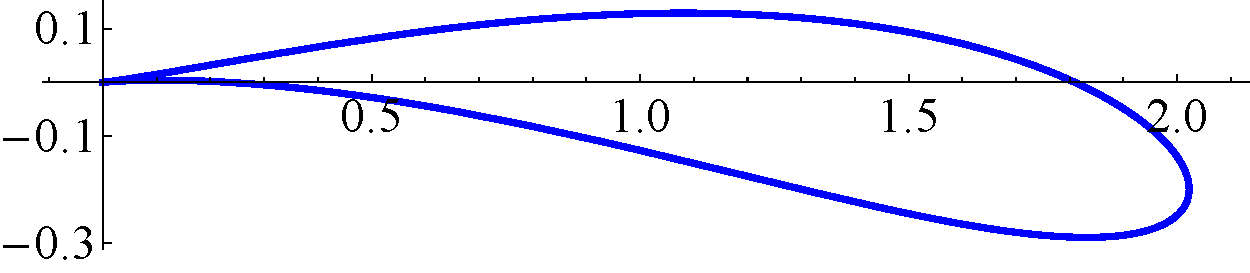
\includegraphics[width=0.55\textwidth]{figWing}
	\caption{Профиль Жуковского с параметрами $a=1$, $\eta= 1.15$, $\alpha=\pi/30$}
	\label{figZhuk}
\end{figure}

Ниже приведены точные значения всех компонент симметричной матрицы присоединенных масс. Примем обозначение $\sigma = \eta/(2\eta\cos\alpha - 1)$, $\rho$ "--- плотность среды,~\cite{Sedov}:
\begin{gather*}
	\lambda^{\mathrm{ex}}_{11} = \frac{\pi \rho a^2}{4}\bigl(\sigma^2 + \eta^2 - 2\cos2\alpha\bigr), \quad
	\lambda^{\mathrm{ex}}_{22} = \frac{\pi \rho a^2}{4}\bigl(\sigma^2 + \eta^2 + 2\cos2\alpha\bigr), \quad
	\lambda^{\mathrm{ex}}_{12} = \frac{\pi \rho a^2}{2}\sin 2\alpha, \\
	\lambda^{\mathrm{ex}}_{16} = \frac{\pi \rho a^3}{8} \sin\alpha \bigl( \sigma^2 + \eta^2 + 4(\sigma+\eta)\cos\alpha \bigr), \\
	\lambda^{\mathrm{ex}}_{26} = \frac{\pi \rho a^3}{8} \bigl( \sigma^3 + \eta^3 + ( \sigma^2 + \eta^2)\cos\alpha  + 2(\sigma+\eta)\cos2\alpha \bigr),\\
	\lambda^{\mathrm{ex}}_{66} = \frac{\pi \rho a^4}{8} \sigma^2 \eta^2 \bigl( 8\sigma^2 \eta^2 \cos^4\alpha - 2 \sigma \eta \sin^2 2\alpha + \cos4\alpha \bigr).
\end{gather*}

Используя точные значения присоединенных масс и моментов инерции, можно вычислить значения ошибок, возникающих при использовании формул~\eqref{addmass}--\eqref{addmoment}, в~зависимости от количества панелей, на которые разбивается исходный профиль, и используемой численной схемы.

Будем считать плотность среды $\rho=1$, а ошибку как максимум отношения разности точного и полученного численного решения к точному значению:
\[
 \delta\lambda_{ij}=\max_{i,j}{\left(\frac{|\lambda^{\mathrm{ex}}_{ij}-\lambda_{ij}|}{\lambda^{\mathrm{ex}}_{ij}}\right)}.
\]
Тогда результаты можно обобщить в таблицу ниже для всех описанных ранее схем с кусочно-постоянным, кусочно-линейным и асимптотическим представлениями решения в зависимости от количества панелей для неограниченного решения относительно интенсивности вихревого слоя на поверхности профиля.\bigskip
\begin{table}[!h]
	\label{errors}
	\centering		
	\caption{Ошибки при вычислении присоединенных масс}\medskip	
	\begin{tabular}{|c|c|c|c|c|c|c|}		
		\hline
		$n$ & 100 & 200 & 400 & 800 & 1600 & 3200 \\\hline
		$\mathcal{T}^0$ & $0.025092$ & $0.012923$ & $0.006885$ & $0.003729$ & $0.002034$ & $0.001112$ \\\hline
		$\mathcal{T}^1$ & $0.004551$ & $0.001652$ & $0.000739$ & $0.000351$ & $0.000171$ & $0.000085$ \\
		\hline
		$\mathcal{T}^1_{a}$ & $0.004587$ & $0.001189$ &  $0.000301$ & $0.000076$ & $0.000019$ & $4.74\times10^{-6}$ \\\hline
		$\mathcal{T}^1_{aMOD}$ & $0.003705$ & $0.000960$ &  $0.000243$ & $0.000061$ & $0.000015$ & $3.84\times10^{-6}$ \\
		\hline
	\end{tabular}
\end{table}	
 
 Приведем таблицу порядков сходимости численного решения по отношению к точному неограниченному решению.

\begin{table}[!h]
	\centering	
	\caption{Порядки сходимости схем}\medskip					
	\begin{tabular}{|c|c|c|c|c|c|c|}
		\hline
		$n$ & 100 & 200 & 400 & 800 & 1600 & 3200 \\ \hline
		$\mathcal{T}^0$ & $1.19$ & $0.96$ & $0.91$ & $0.88$ & $0.87$ & $0.87$\\
		\hline
		$\mathcal{T}^1$ & $1.91$ & $1.46$ & $1.16$ & $1.08$ & $1.03$ & $1.01$\\
		\hline
		$\mathcal{T}^1_{a}$ & $1.91$ & $1.95$ & $1.98$ & $1.99$ & $2.00$ & $2.00$ \\
		\hline
		$\mathcal{T}^1_{aMOD}$ & $1.91$ & $1.95$ & $1.98$ & $1.99$ & $2.00$ & $2.00$\\
		\hline
	\end{tabular}
\end{table}

Из таблиц выше можно сделать вывод, что на неограниченных решениях кусочно-постоянная  кусочно-линейная схемы теряют свои порядки точности, а две схемы с~асимптотическим представлением решения позволяют учесть особенность решения и~получить результаты для присоединенных масс с~желаемым 2-м порядком точности. Однако введение новой проекционной функции, как это было сделано в схеме $\mathcal{T}^1_{aMOD}$, не представляется рациональным, поскольку, как видно из результатов обеих таблиц, данная схема сходится почти так же как и схема $\mathcal{T}^1_a$. Следовательно, для вычислений более удобным будет использование схемы $\mathcal{T}^1_a$.

\section{Программная реализация расчетных схем}

\looser{-0.02}{Описанные численные схемы для получения численного решения граничного} интегрального уравнения~\eqref{Tscheme} \looser{-0.02}{были реализованы с помощью системы Wolfram Mathematica}. Модули программ написаны с целью нахождения как самого решения относительно интенсивности вихревого слоя, так и расчета присоединенных масс и моментов инерции одного гладкого профиля. Примером такого профиля был выбран профиль Жуковского. Данный выбор обусловлен тем, что для текущей постановки задачи все точные аналитические решения известны. 

Каждый модуль состоит из нескольких тематических блоков:
\begin{enumerate}
	\item разбиение профиля по панелям равной длины;
	\item выполнение расчетов всех компонент векторов и матриц, составляющих схемы \eqref{sys1}, \eqref{sys1asymp}, \eqref{sys1asymplight};
	\item решение получаемых линейных систем, нахождение решения для интенсивности вихревого слоя обтекаемого профиля;
	\item нахождение компонент матрицы присоединенных масс;
	\item оценка значений присоединенных моментов и масс: вычисление относительных погрешностей вычисления.
\end{enumerate}

\looser{-0.01}{Из-за больших вычислительных нагрузок, связанных с увеличением числа панелей профиля, получать  линейные системы алгебраических уравнений напрямую средствами Wolfram Mathematica становится весьма трудоемкой операцией. С целью оптимизации написанного кода была создана внутренняя библиотека, использующая методы для вычисления компонент матриц и всех интегралов, написанные на языке C++}.
\section-{Заключение}
Таким образом, в ходе выполнения курсовой работы была реализована расчетная $T$-схема с кусочно-постоянным, кусочно-линейным и асимптотическими представлениями решения для плоского обтекания гладкого профиля. Результаты работы расчетной схемы были проверены для профиля Жуковского, а также были проведены сравнения численных решений с известными точными.

Далее была изучена задача о вычислении присоединенных масс и моментов инерции крылового профиля по полученным решениям для интенсивности вихревого слоя. Полученные значения сравнивались также с известными точными.

Все описанные подходы реализованы в Wolfram Mathematica с демонстрацией результатов работы.

\begin{thebibliography}{10}
\bibitem{Kempka} Kempka S.N., Glass M.W., Peery J.S., Strickland J.H., Ingber M.S. Accuracy considerations for implementing velocity boundary conditions in vorticity formulations // SANDIA report. SAND96-0583, UC-700. 1996. 52 p.
\bibitem{Lifanov} Лифанов И.К. Метод сингулярных интегральных уравнений и численный эксперимент (в математической физике, аэродинамике, теории упругости и дифракции волн). М.: ТОО <<Янус>>, 1995. 520 с.
\bibitem{MM} Кузьмина К.С., Марчевский И.К., Морева В.С. Определение интенсивности вихревого слоя при моделировании вихревыми методами обтекания профиля потоком несжимаемой среды // Математическое моделирование. 2017. Т.~29, №~10. C.~20--34.
\bibitem{PMM} Кузьмина К.С., Марчевский И.К. О вычислении влияния вихревого слоя и точечных вихрей при приближенном решении граничного интегрального уравнения в двумерных вихревых методах вычислительной гидродинамики // Прикладная математика и механика. 2019. Т.~83, №~3. С.~495--508.
\bibitem{Fletcher} Флетчер К. Численные методы на основе метода Галеркина. М.: Мир, 1988. 352~с.
\bibitem{Exact} Kuzmina K.S., Marchevsky I.K., Ryatina E.P. Exact solutions of boundary integral equation arisingin vortex methods for incompressible flow simulation around elliptical and Zhukovsky airfoils //Journal of Physics: Conf. Series. 2019. Vol.~1348. Art.~012099.
\bibitem{Sedov} Седов Л.И. Плоские задачи гидродинамики и аэродинамики. М.-Л., ГИТТЛ, 1950. 443 с.
\bibitem{Dyn2019} Дынникова Г.Я. О присоединенной массе в модели вязкой несжимаемой жидкости // Доклады РАН. 2019. Т.~488, №~5. С.~493--497.
\bibitem{Miln} Милн-Томсон Л. Теоретическая гидродинамика. М.: Мир, 1964. 660 с.
\bibitem{Marchevskii} Марчевский И.К. Разработка и реализация $T$-схем численного решения граничных интегральных уравнений в математических моделях вихревых методов вычислительной гидродинамики: дис. \ldots д-ра физ.-мат. наук. М., 2021. 480 с.
\end{thebibliography}

\end{document} 